% 编译：在 documents/ 目录里运行 xelatex report.tex 两遍（中间产物输出到 build/）
\documentclass[12pt,a4paper,fontset=windows]{ctexart}

\usepackage{geometry}
\geometry{left=2.4cm,right=2.4cm,top=2.4cm,bottom=2.4cm}
\usepackage{graphicx}
\usepackage{booktabs}
\usepackage{colortbl}
\usepackage{array}
\usepackage{longtable}
\usepackage{float}
\usepackage{caption}
\usepackage{enumitem}
\usepackage{xcolor}
\usepackage{amsmath}
\usepackage{amssymb}
\usepackage{amsthm}
\usepackage{listings}
\usepackage{tikz}
\usetikzlibrary{arrows.meta,positioning,calc}
\usepackage[nobottomtitles*]{titlesec}
\usepackage[hidelinks]{hyperref}

\setmainfont{Times New Roman}
\setmonofont{Consolas}
% 中文引号按 CJK 标点处理，防止 xeCJK 在引号与汉字间插入西文间距
\xeCJKDeclareCharClass{CJK}{"2018, "2019, "201C, "201D}

% PR 互评匿名阶段：封面、分工、PDF 元数据一律不含姓名、学号、真实组号与环境标识
\hypersetup{
  pdftitle={Shopping With Coupons: Heap Merging and Value-Domain Binary Search},
  pdfauthor={},
  pdfsubject={},
  pdfkeywords={},
  pdfcreator={},
  pdfcreationdate={D:20261123184500+08'00'},
  pdfmoddate={D:20261123184500+08'00'}
}

% 章标题沿用课程要求格式：Chapter N: Title，下配细横线分隔
\titleformat{\section}{\raggedright\bfseries\fontsize{14}{17}\selectfont}{Chapter \thesection:}{0.85em}{}[{\color{black}\titlerule[0.9pt]}]
\titlespacing*{\section}{0pt}{1.35em}{0.65em}
\titleformat{\subsection}{\raggedright\bfseries\fontsize{12}{15}\selectfont}{\thesubsection}{0.7em}{}[{\color{black}\titlerule[0.4pt]}]
\titlespacing*{\subsection}{0pt}{1.15em}{0.5em}
\titleformat{\subsubsection}{\raggedright\bfseries}{\thesubsubsection}{0.6em}{}

\theoremstyle{plain}
\newtheorem{theorem}{定理}

\lstdefinestyle{pseudo}{
  basicstyle=\ttfamily\small,
  columns=fullflexible,
  keepspaces=true,
  frame=single,
  framerule=0.4pt,
  rulecolor=\color{gray!45},
  backgroundcolor=\color{gray!5},
  xleftmargin=0.5em,
  xrightmargin=0.5em,
  aboveskip=0.55em,
  belowskip=0.55em,
  breaklines=true,
  escapeinside={(*@}{@*)}
}
\lstset{style=pseudo}

\newcommand{\code}[1]{\texttt{#1}}
\newcommand{\tabhead}[1]{\textbf{#1}}

\pagestyle{plain}
\setlength{\parindent}{0pt}
\setlength{\parskip}{0.46em}
\setlength{\emergencystretch}{2em}

\begin{document}

%=====================================================================
% 封面页（PR 匿名版）
%=====================================================================
\begin{titlepage}
\centering
\vspace*{1.6cm}
{\fontsize{13}{16}\selectfont Advanced Data Structures and Algorithm Analysis --- Project 5\par}

\vspace{1.2cm}
{\bfseries\fontsize{24}{31}\selectfont Shopping With Coupons:\par}
\vspace{0.45em}
{\bfseries\fontsize{20}{27}\selectfont Heap Merging and Value-Domain Binary Search\par}

\vspace{1.8cm}
{\bfseries\fontsize{16}{20}\selectfont Member A\hspace{2.2em}Member B}

\vspace{0.8cm}
{\fontsize{12}{15}\selectfont Group: [Anonymous for Peer Review]}

\vspace{1.0cm}
{\bfseries\fontsize{13}{16}\selectfont Date: 2026-11-23}
\end{titlepage}

%=====================================================================
\section{Introduction}

\subsection{题目要求}

商店里有 $N$ 种商品，价格为正整数 $p_1, p_2, \dots, p_N$；手头同时有 $N$ 种优惠券，面值为正整数 $c_1, c_2, \dots, c_N$，另有总预算 $D$ 元。购买规则满足四条约束：

\begin{enumerate}[leftmargin=1.8em,itemsep=0.12em,topsep=0.18em]
  \item 每种商品可以购买多次，每种优惠券也可以使用多次；
  \item 每次购买一件商品恰好使用一张优惠券，实际支付金额为 $p_i - c_j$；
  \item 同一个「商品--优惠券」配对 $(i, j)$ 最多只能使用一次，全过程共有 $N^2$ 种互不重复的合法购买选项；
  \item 数据保证 $\max_j c_j < \min_i p_i$，且输入满足 $1 \le N \le 10^5$、$0 \le D \le 10^6$、$1 \le c_j < p_i \le 10^9$（题面主约束为正整数 $D$，测试中一并覆盖 $D=0$ 退化边界）。
\end{enumerate}

目标是在总花费不超过 $D$ 的前提下，先最大化购买件数 $K$，再在买满 $K$ 件的前提下最大化剩余金额 $R$。以样例 $N=4, D=30$、价格 $\{12, 20, 15, 10\}$、优惠券 $\{9, 6, 8, 7\}$ 为例：10 元商品配齐四张券花去 10 元，12 元商品配 9、8、7 三张券花去 12 元，再以 9 元券买入一件 15 元商品花去 6 元，共买 8 件、剩 2 元。

\subsection{这份报告做了什么}

直接把 $N^2$ 种配对展开排序，在 $N=10^5$ 时会产生 $10^{10}$ 个元素，单存储就需要约 74.5~GiB 内存，无法运行。解决这个问题的关键在于利用 $p_i - c_j$ 的二维单调结构，在不展开矩阵的前提下直接定位最便宜的前 $K$ 个配对。

本报告在同一代码框架下实现并对比了四种递进算法（暴力展开、标准 $N$ 路归并堆、前沿懒扩展堆、值域二分双指针），主要回答三个问题：在题面约束下哪类算法更快、排名随购买件数 $K$ 如何变化；当预算 $D$ 突破题面 $10^6$ 上限后，两类堆与值域二分的差距在哪里拉开；以及这些实测结论各自成立的边界是什么。

后面三章按此展开：第 2 章做数学建模、贪心证明并给出四种算法的设计与伪代码；第 3 章展示正确性对拍、排查记录和四组基准实验结果；第 4 章推导时空复杂度，按排序、求解与单步代价拆解实测读数，并补充两类常见题面变体的对比。

%=====================================================================
\section{Data Structure / Algorithm Specification}

\subsection{数学建模与贪心正确性}

将商品价格升序排为 $p_0 \le p_1 \le \dots \le p_{N-1}$，优惠券面值降序排为 $c_0 \ge c_1 \ge \dots \ge c_{N-1}$，定义 $N \times N$ 的虚拟实付价格矩阵：
\[
M[i][j] = p_i - c_j, \qquad 0 \le i, j < N.
\]
因为 $\max_j c_j < \min_i p_i$，矩阵所有元素满足 $M[i][j] \ge 1$。同时 $p_i$ 随行号不降、$-c_j$ 随列号不降，$M$ 是一张行和列同时单调不降的矩阵。

原问题等价于选出子集 $S \subseteq \{0,\dots,N-1\}^2$，在 $\sum_{(i,j)\in S} M[i][j] \le D$ 下使 $(|S|,\ D-\sum_{(i,j)\in S} M[i][j])$ 字典序最大。

\begin{theorem}[贪心选择性质与双目标统一]
将矩阵 $M$ 的全部 $N^2$ 个实付价格按不降顺序记为 $w_1 \le w_2 \le \dots \le w_{N^2}$。设 $K$ 为满足 $\sum_{t=1}^{K} w_t \le D$ 的最大整数（若 $w_1 > D$ 则 $K=0$），则最优购买件数必为 $K$，最优剩余金额必为 $R = D - \sum_{t=1}^{K} w_t$。
\end{theorem}

\begin{proof}
采用交换论证\cite{clrs2022}。任取一个大小为 $k$ 的合法方案 $S$，将其元素升序排为 $s_1 \le s_2 \le \dots \le s_k$。由于 $w_1, \dots, w_k$ 是全矩阵中最小的 $k$ 个数，对任意 $t \in \{1, \dots, k\}$ 均有 $w_t \le s_t$，故
\[
\sum_{t=1}^{k} w_t \le \sum_{t=1}^{k} s_t \le D.
\]
若 $k > K$，由 $K$ 的最大性必有 $\sum_{t=1}^{k} w_t > D$，矛盾。因此合法方案件数至多为 $K$。在 $k=K$ 时，上式同时说明任何 $K$ 元方案的总花费都不小于 $\sum_{t=1}^{K} w_t$，剩余金额至多为 $D - \sum_{t=1}^{K} w_t$。选取前 $K$ 小配对同时达到两项上界。
\end{proof}

由 $M[i][j] \ge 1$ 可立即得到购买件数的上界：
\[
K \le \min(N^2, D).
\]
在题面约束 $N \le 10^5$、$D \le 10^6$ 下，$N^2 = 10^{10}$，但 $K$ 不会超过 $10^6$。这也是优先队列在题面范围内可行的原因。一旦把预算放宽到 $D = 10^{12}$ 以上，$K$ 跨过亿级，逐件弹出的算法就会失效。

\subsection{四种算法总览与公平比较设计}

围绕摆脱 $N^2$、压缩堆内无效元素、摆脱 $K$ 三步递进，我们在源码文件 \code{solvers.cpp} 中实现了四个求解器，总览见表~\ref{tab:algo_overview}。

\begin{table}[htbp]
\centering
\caption{四个求解器的设计定位与理论复杂度总览（$V = M_{\max} - M_{\min} + 1$ 为实付价整数跨度）}
\label{tab:algo_overview}
\footnotesize
\setlength{\tabcolsep}{3.4pt}
\begin{tabular}{@{}l>{\raggedright\arraybackslash}p{3.0cm}l>{\raggedright\arraybackslash}p{2.3cm}>{\raggedright\arraybackslash}p{2.5cm}@{}}
\toprule
\rowcolor{gray!12}\tabhead{标识} & \tabhead{核心范式} & \tabhead{时间复杂度} & \tabhead{总空间复杂度} & \tabhead{主要依赖参数} \\
\midrule
\code{brute}      & 展开全部 $N^2$ 配对排序 & $O(N^2 \log N)$ & $O(N^2)$ & 仅受限于 $N$ \\
\code{heap\_full} & $N$ 路归并堆（全行首入堆） & $O(N\log N + K\log N)$ & $O(N)$ & 强依赖 $K$ \\
\code{heap\_lazy} & 网格前沿懒扩展最小堆 & $O(N\log N + K\log\min(N,K))$ & $O(N)$（堆 $O(\min(N,K))$） & 依赖 $K$，$K\ll N$ 占优 \\
\code{bsearch}    & 值域二分 + 单调双指针 & $O(N\log N + N\log(\min(V,D)+1))$ & $O(N)$ & 与 $K$ 无关，适合大预算 \\
\bottomrule
\end{tabular}
\end{table}

公平对比依赖两项工程约束。第一，四个求解器共享只读原始数组 \code{const vector<long long>\&}，各自拷贝后再排序；如果不拷贝而原地排序，同一批次中后面的算法面对的就是已排序数组，测出的耗时差就说不清是算法带来的，还是预处理带来的。第二，两类堆共用同一份手写 1-indexed 二叉最小堆 \code{MinHeap}（空穴法调整 + 原地替换 \code{replaceTop}）；如果一边用 \code{std::priority\_queue}、另一边手写堆，容器常数就会遮住扩展策略本身的差异。

\subsection{朴素暴力与两类最小堆归并}

\subsubsection{朴素展开排序（\texorpdfstring{\code{brute}}{brute}）}

枚举全部 $N^2$ 对 $(i,j)$ 算出 $p_i - c_j$，调用 \code{std::sort} 升序排列后顺序扣减预算直至停机。该实现直接按定理~1 的定义计算，不依赖任何矩阵单调性或收尾公式，在 $N \le 4000$ 上作为独立真值基准参与对拍；对 $N > 4000$ 主动拒绝执行以防内存溢出。

\subsubsection{标准 \texorpdfstring{$N$}{N} 路归并最小堆（\texorpdfstring{\code{heap\_full}}{heap\_full}）}

排序后，矩阵每一行 $r$ 都是一条升序序列 $p_r - c_0 \le \dots \le p_r - c_{N-1}$，问题直接归约为经典的多路归并\cite{knuth1998}。算法初始将全部 $N$ 个行首 $(p_r - c_0, r, 0)$ 装入最小堆，每轮取出堆顶扣减预算并推入同行下一列。

实现里有两处减常数处理。因为 $p_0 \le \dots \le p_{N-1}$，初始 $N$ 个行首本身已经有序，顺序写入 1-indexed 数组后天然满足小根堆性质，只需 $O(N)$ 拷贝而不必逐个上滤。同行右移时直接调用 \code{replaceTop} 覆写堆顶后单趟下沉，省掉一次 \code{pop} 加 \code{push} 的往返。但当 $K \ll N$ 时，它依然要先装满 $N$ 个行首，且后续每次下沉的堆高始终接近 $\log_2 N$。

\begin{lstlisting}[float=htbp, title={算法 1：标准 $N$ 路归并最小堆（\code{heap\_full}）}]
sort p ascending;  sort c descending
for r <- 0 to N - 1:
    heap.appendSorted((p[r] - c[0], r, 0))   // 行首已有序，O(N) 直接成堆
cnt <- 0;  rem <- D
while not heap.empty():
    (val, r, col) <- heap.top()
    if val > rem: break
    rem <- rem - val;  cnt <- cnt + 1
    if col + 1 < N: heap.replaceTop((p[r] - c[col + 1], r, col + 1))
    else:           heap.pop()
return (cnt, rem)
\end{lstlisting}

\subsubsection{前沿懒扩展最小堆（\texorpdfstring{\code{heap\_lazy}}{heap\_lazy}）}

为消除 $K \ll N$ 时的初始装载冗余，我们将网格组织成以 $(0,0)$ 为根的有向生成树：对任意非根格子 $(r, col)$，定义唯一父结点为
\[
\text{parent}(r, col) =
\begin{cases}
(r - 1, 0), & col = 0 \text{ 且 } r > 0,\\
(r, col - 1), & col > 0.
\end{cases}
\]
由矩阵行列单调性，子结点的实付价不小于父结点，父结点必先于子结点出堆。初始仅压入 $(0,0)$；每次弹出 $(r, col)$ 后，向右推 $(r, col+1)$，仅当 $col=0$ 时额外向下推 $(r+1, 0)$。每个格子恰有唯一父结点，既不漏也不重，无需哈希表去重（图~\ref{fig:matrix_views}(a)）。

\begin{lstlisting}[float=htbp, title={算法 2：前沿懒扩展最小堆（\code{heap\_lazy}）}]
sort p ascending;  sort c descending
heap.push((p[0] - c[0], 0, 0));  cnt <- 0;  rem <- D
while not heap.empty():
    (val, r, col) <- heap.top()
    if val > rem: break
    rem <- rem - val;  cnt <- cnt + 1
    hasRight <- (col + 1 < N);  hasDown <- (col == 0 and r + 1 < N)
    if hasRight and hasDown:
        heap.replaceTop((p[r] - c[col + 1], r, col + 1))
        heap.push((p[r + 1] - c[0], r + 1, 0))
    else if hasRight: heap.replaceTop((p[r] - c[col + 1], r, col + 1))
    else if hasDown:  heap.replaceTop((p[r + 1] - c[0], r + 1, 0))
    else:             heap.pop()
return (cnt, rem)
\end{lstlisting}

\begin{figure}[htbp]
\centering
\begin{tikzpicture}[scale=0.80, >=Stealth, font=\small]
%---- 左子图：(a) 懒扩展无重生成树 ----
\begin{scope}[shift={(0,0)}]
  \node[font=\bfseries\small] at (2.0, 5.15) {(a) 前沿懒扩展生成树};
  \foreach \r/\val in {0/p_0,1/p_1,2/p_2,3/p_3} {
    \node[left, font=\footnotesize] at (-0.08, 3.5-\r) {$\val$};
  }
  \foreach \c/\val in {0/-c_0,1/-c_1,2/-c_2,3/-c_3} {
    \node[above, font=\footnotesize] at (0.5+\c, 4.06) {$\val$};
  }
  \fill[blue!14] (0,3) rectangle (3,4);
  \fill[blue!14] (0,2) rectangle (2,3);
  \fill[blue!14] (0,1) rectangle (1,2);
  \fill[orange!28] (3,3) rectangle (4,4);
  \fill[orange!28] (2,2) rectangle (3,3);
  \fill[orange!28] (1,1) rectangle (2,2);
  \fill[orange!28] (0,0) rectangle (1,1);
  \draw[step=1.0, gray!60] (0,0) grid (4,4);
  \foreach \y in {3.5,2.5,1.5} {
    \draw[->, thick, blue!70!black] (0.5,\y) -- (0.5,\y-0.88);
  }
  \draw[->, thick, blue!70!black] (0.62,3.5) -- (1.42,3.5);
  \draw[->, thick, blue!70!black] (1.62,3.5) -- (2.42,3.5);
  \draw[->, thick, orange!80!black] (2.62,3.5) -- (3.42,3.5);
  \draw[->, thick, blue!70!black] (0.62,2.5) -- (1.42,2.5);
  \draw[->, thick, orange!80!black] (1.62,2.5) -- (2.42,2.5);
  \draw[->, thick, orange!80!black] (0.62,1.5) -- (1.42,1.5);
  \node[font=\footnotesize, align=center] at (2.0,-0.55) {浅蓝: 已弹出 \quad 浅橙: 堆内前沿};
\end{scope}

%---- 右子图：(b) 值域二分双指针阶梯 ----
\begin{scope}[shift={(7.4,0)}]
  \node[font=\bfseries\small] at (2.0, 5.15) {(b) 值域二分单调阶梯};
  \foreach \r/\val in {0/p_0,1/p_1,2/p_2,3/p_3} {
    \node[left, font=\footnotesize] at (-0.08, 3.5-\r) {$\val$};
  }
  \foreach \c/\val in {0/-c_0,1/-c_1,2/-c_2,3/-c_3} {
    \node[above, font=\footnotesize] at (0.5+\c, 4.06) {$\val$};
  }
  \fill[teal!16] (0,3) rectangle (4,4);
  \fill[teal!16] (0,2) rectangle (3,3);
  \fill[teal!16] (0,1) rectangle (1,2);
  \draw[step=1.0, gray!60] (0,0) grid (4,4);
  \draw[very thick, teal!75!black] (4,4) -- (4,3) -- (3,3) -- (3,2) -- (1,2) -- (1,1) -- (0,1) -- (0,0);
  \node[teal!65!black, font=\footnotesize\bfseries] at (1.5,3.5) {$\le T$};
  \node[gray!75!black, font=\footnotesize] at (2.9,1.5) {$> T$};
  \draw[->, thick, red!75!black] (3.85,2.7) -- (3.15,2.7);
  \draw[->, thick, red!75!black] (2.85,1.7) -- (1.15,1.7);
  \node[font=\footnotesize, align=center] at (2.0,-0.55) {指针 $j$ 随行递增单调左移，$O(N)$ 扫完};
\end{scope}
\end{tikzpicture}
\caption{行列单调实付价矩阵 $M[i][j]=p_i-c_j$ 在两类高效算法下的操作几何视图}
\label{fig:matrix_views}
\end{figure}

\subsection{值域二分与单调双指针}

两类堆每次只买一件，时间下界无法低于 $\Omega(K)$。改为在实付价格阈值 $T$ 上二分，就能一次性计入所有 $M[i][j] \le T$ 的配对。

预先对降序数组 $c$ 计算前缀和 $\mathrm{prefC}[m] = \sum_{t=0}^{m-1} c_t$。对任意阈值 $T$，记
\[
\mathrm{cnt}(T) = \big|\{(i,j) : p_i - c_j \le T\}\big|, \qquad
\mathrm{sum}(T) = \sum_{p_i - c_j \le T} (p_i - c_j).
\]
当行号 $i$ 从 $0$ 增至 $N-1$ 时，$p_i$ 不降，满足 $p_i - c_j \le T$ 的最大列下标 $j$ 单调不增（图~\ref{fig:matrix_views}(b)）。维护 $j$ 从 $N-1$ 单调左移，第 $i$ 行有 $m = j+1$ 个配对不超过 $T$，其总花费可在 $O(1)$ 内算成 $m \cdot p_i - \mathrm{prefC}[m]$。扫描中再加两条剪枝：遇到 $p_i - c_0 > T$ 时立即 \code{break}，累计花费超过 $D$ 时早停返回 \code{false}。

位宽上，当 $N=10^5, p_i \le 10^9$ 时，全矩阵总花费最高可达 $10^{19}$，超出 64 位有符号整数上限（约 $9.22 \times 10^{18}$）。因此前缀和与累加均采用 \code{\_\_int128}。进入二分前，先用 $O(1)$ 判掉 $M_{\min} > D$ 的零购买边界，再用 $O(N)$ 闭式公式 $N\sum p_i - N\sum c_i$ 判掉全矩阵 $N^2$ 件买光的边界。

剩余情形满足 $M_{\min} \le D < \mathrm{sum}(M_{\max})$。将二分搜索区间设在 $[M_{\min},\ \min(M_{\max}-1,\ D)]$，求出满足 $\mathrm{sum}(T) \le D$ 的最大整数 $T^*$（若 $\mathrm{sum}(M_{\min}) > D$ 则记 $T^* = M_{\min}-1$）。临界价位 $T^*+1$ 上可能存在大量重复配对，收尾正确性由下述定理保证：

\begin{theorem}[重复值收尾与上界收紧]
在排除零购买与全买光后，令 $H = \min(M_{\max}-1,\ D)$，$T^*$ 为 $[M_{\min}, H]$ 中满足 $\mathrm{sum}(T) \le D$ 的最大整数（若无则取 $M_{\min}-1$）。记剩余预算 $R_0 = D - \mathrm{sum}(T^*)$，则原问题最优解恒为
\[
K = \mathrm{cnt}(T^*) + \left\lfloor \frac{R_0}{T^* + 1} \right\rfloor, \qquad
R = R_0 \bmod (T^* + 1).
\]
\end{theorem}

\begin{proof}
分两种情况。情况一：$\mathrm{sum}(T^* + 1) > D$（当 $T^* < H$ 或 $H = M_{\max}-1$ 时必成立）。设矩阵中实付价恰好等于 $T^*+1$ 的配对共有 $q$ 个，则
\[
q \cdot (T^* + 1) = \mathrm{sum}(T^* + 1) - \mathrm{sum}(T^*) > D - \mathrm{sum}(T^*) = R_0.
\]
因 $T^*+1 \ge 1$ 且 $q$ 为整数，必有 $q \ge \lfloor R_0 / (T^*+1) \rfloor + 1$。即价位为 $T^*+1$ 的配对一定足够补买 $\Delta = \lfloor R_0/(T^*+1) \rfloor$ 件；买完后余钱 $R_0 \bmod (T^*+1) < T^*+1$，再也买不起任何剩余配对。

情况二：$T^* = H = D < M_{\max}-1$ 且 $\mathrm{sum}(D+1) \le D$（对应价格在 $D$ 附近出现大断层）。此时所有 $\le D$ 的配对已全部买入，剩余未买配对价格均 $\ge D+1 > D \ge R_0$，一件也买不起。而公式算出 $\lfloor R_0/(D+1) \rfloor = 0$、$R_0 \bmod (D+1) = R_0$，与真实最优解一致。
\end{proof}

由于闭区间 $[M_{\min}, H]$ 最多包含 $L = \min(V-1,\ D - M_{\min} + 1) \le \min(V, D)$ 个候选整数（其中 $V = M_{\max}-M_{\min}+1 \ge 1$），二分轮数至多为 $\lceil \log_2(\min(V, D)+1) \rceil$ 轮。当矩阵全相等时 $V=1$、$H < M_{\min}$，循环执行 0 轮后直接进入收尾公式。完整伪代码见算法~3。

\begin{lstlisting}[float=htbp, title={算法 3：值域二分 + 单调双指针 + 前缀和（\code{bsearch}）}]
function checkBudget(T):
    j <- N - 1;  sum <- 0                       // 128 位累加防溢出
    for i <- 0 to N - 1:
        if p[i] - c[0] > T: break               // 后续行最小实付价均超过 T
        while j >= 0 and p[i] - c[j] > T: j <- j - 1
        m <- j + 1;  sum <- sum + m * p[i] - prefC[m]
        if sum > D: return false                // 超预算早停
    return true

sort p ascending;  sort c descending;  build prefC
if p[0] - c[0] > D: return (0, D)
totalAll <- N * sum(p) - N * prefC[N]
if totalAll <= D: return (N * N, D - totalAll)

lo <- p[0] - c[0];  hi <- min(p[N - 1] - c[N - 1] - 1, D);  bestT <- lo - 1
while lo <= hi:
    mid <- lo + floor((hi - lo) / 2)
    if checkBudget(mid): bestT <- mid;  lo <- mid + 1
    else:                hi <- mid - 1
(cnt, sum) <- fullTwoPointerCountAndSum(bestT)  // 对 bestT 完整扫一次取精确 cnt 与 sum
rem0 <- D - sum;  nextP <- bestT + 1
return (cnt + floor(rem0 / nextP), rem0 mod nextP)
\end{lstlisting}

%=====================================================================
\section{Testing Results}

\subsection{实验环境与计时口径}

全部编译、对拍与测速在同一台 64 位 Windows 主机上完成，使用 GCC（C++17）以固定编译参数 \code{-O2 -std=c++17 -Wall -Wextra} 构建，零警告通过。输入读取采用标准 C 文件流快读，计时沿用标准库 \code{clock()}（本机 \code{CLOCKS\_PER\_SEC = 1000}，滴答粒度 1~ms）。

为压低 1~ms 量化误差与系统调度抖动，\code{coupons bench} 对每组输入重复执行 \code{repeat} 次并取均值，每次重复都传入未排序原始数组。重复次数按单次耗时分档设置：实验族 A 中 \code{brute} 取 5 次（$N=1000$）与 3 次（$N=2000$），其余三个算法按规模从 $N=1000$ 到 $10^5$ 依次取 50、30、30、25、15、10、10 次；实验族 B 均取 10 次；实验族 C 常规分布取 10 次，较快的 \code{D3}/\code{D4} 取 15 次；实验族 D 在 $D=10^6,10^7,10^{12},10^{14}$ 取 10 次，$D=10^8$ 全算法取 5 次，$D=10^{10}$ 全算法取 2 次。

口径局限先交代两处：一是毫秒数仅在本机、本批次、固定 \code{-O2} 下横向可比，换机器、换系统负载或换优化级别后绝对值都会变化；二是对单次低于 0.05~ms 的极小用例，重复 50 次仍可能触及滴答下限，此时需以与机器无关的操作计数 \code{ops} 和轮数 \code{rounds} 为主。

\subsection{功能测试、边界用例与四层自动对拍}

主程序通过 \code{coupons test} 内置 360 组自动校验。第一层为 10 组手工边界用例，全部四算法一致通过，详见表~\ref{tab:fixed_cases}。

\begin{table}[htbp]
\centering
\caption{手工功能与边界测试用例汇总（四算法逐项校验一致）}
\label{tab:fixed_cases}
\footnotesize
\setlength{\tabcolsep}{3.0pt}
\begin{tabular}{@{}l>{\raggedright\arraybackslash}p{4.9cm}lll@{}}
\toprule
\rowcolor{gray!12}\tabhead{用例} & \tabhead{测试目的与输入（$p;\ c;\ D$）} & \tabhead{期望} & \tabhead{实际} & \tabhead{状态} \\
\midrule
\code{T01\_sample} & 题面样例：$\{12,20,15,10\};\ \{9,6,8,7\};\ 30$ & \code{8 2} & \code{8 2} & 通过 \\
\code{T02\_single} & $N=1$ 且余额清零：$\{100\};\ \{99\};\ 1$ & \code{1 0} & \code{1 0} & 通过 \\
\code{T03\_zero} & 零购买边界：$\{10,12,15\};\ \{5,4,3\};\ 4$ & \code{0 4} & \code{0 4} & 通过 \\
\code{T04\_all} & 买光全矩阵：$\{10,12\};\ \{9,8\};\ 100$ & \code{4 90} & \code{4 90} & 通过 \\
\code{T05\_eq\_part} & 全等平地不整除：$\{10\}^4;\ \{7\}^4;\ 20$ & \code{6 2} & \code{6 2} & 通过 \\
\code{T06\_eq\_exact} & 全等平地全买光：$\{10\}^3;\ \{7\}^3;\ 27$ & \code{9 0} & \code{9 0} & 通过 \\
\code{T07\_gap} & 价格大断层测上界收紧：$\{10,1000\};\ \{9,8\};\ 100$ & \code{2 97} & \code{2 97} & 通过 \\
\code{T08\_tie} & 临界价 3 重复三次：$\{10,11,12\};\ \{9,8,7\};\ 10$ & \code{4 2} & \code{4 2} & 通过* \\
\code{T09\_1e9} & 贴近 $10^9$ 上限：$\{10^9{-}i\}_{i=0}^2$; $\{10^9{-}3{-}i\}_{i=0}^2$; $10$ & \code{4 2} & \code{4 2} & 通过* \\
\code{T10\_1e12} & 超大预算全买：$\{10^8{+}\{0,1,5\}\}$; $\{10^8{-}\{1,2,10\}\}$; $10^{12}$ & \code{9 999999999943} & \code{9 999999999943} & 通过* \\
\bottomrule
\end{tabular}

\vspace{0.25em}
{\scriptsize 注：标「*」的三条用例初版手算预期有误，复算后修正预期，四个算法初测输出均与正确值一致（详见 3.3 节）。}
\end{table}

随后 \code{coupons test} 按固定种子 20261123 运行三层自动对拍：
\begin{enumerate}[leftmargin=1.8em,itemsep=0.1em,topsep=0.15em]
  \item \textbf{300 组随机小规模四算法对拍}（$N \in [1, 80]$）：轮换均匀分布、极小值域高重复、大断层、贴近 $10^9$ 四类分布，并穿插 $D=0$ 与买光全矩阵预算，三个高效算法均以独立 \code{brute} 为真值，300/300 全过；
  \item \textbf{30 组中大规模三算法对拍}（$N \in [500, 3000], D \le 10^6$）：两类堆与值域二分逐项一致，30/30 全过；
  \item \textbf{20 组大预算四算法暴力对拍}（$N=300$，$D$ 最高 $10^{13}$、单价最高 $10^9$）：以独立 \code{brute} 直接校验两类堆与 \code{bsearch} 的 \code{\_\_int128} 累加和收尾公式，20/20 全过。
\end{enumerate}

此外，\code{code/samples/} 下四组样例文件经标准输入重定向 \code{coupons < sample.in} 测试，输出与同名 \code{.out} 文件逐字节一致。

\subsection{排查记录：手算预期偏差与短测抖动复核}

测试与基准阶段遇到过两处真实异常。

\textbf{第一处：手算预期出错。}首次编写 \code{T08}、\code{T09} 与 \code{T10} 时，我们在纸上列出 $N=3$ 矩阵的前 4 小实付价 $1,2,2,3$，心算把总和算成了 10（将 \code{T08} 预期余额写成 0、\code{T09} 写成 1），又把 \code{T10} 的全矩阵总花费 57 算成了 54。首次编译运行 \code{coupons test} 立刻停在 \code{T08} 报错：\code{brute 得到 (4,2)，与 expected 的 (4,0) 不一致}。逐格复算确认暴力与三个高效算法均无误，错在手算预期。连 $N=3$ 的小矩阵手算都容易看偏，仅靠手算样例无法保证正确性，必须依赖独立暴力实现充当真值。

\textbf{第二处：短测抖动险些误归因。}初版以 \code{repeat=5} 跑实验族 B 时，\code{K6\_xlarge} 上 \code{heap\_lazy} 曾测出反常高耗时，慢于 \code{heap\_full} 一倍多。当时准备将其归因成「动态扩容叠加首列二次入堆」，但核对操作步数（100.4 万对 110.5 万）发现步数并未反超。随后把各族 \code{repeat} 拉高至 10--50 次重测，\code{heap\_lazy} 在 \code{K6\_xlarge} 落回 2.13~ms，快于 \code{heap\_full} 的 2.53~ms，前次读数实为短测里的单次系统调度毛刺。做性能归因前必须先拿与机器无关的 \code{ops} 核对方向，方向矛盾时先加大重复次数复测。

\subsection{规模扩展与购买量梯度实验}

由 \code{code/tools/gen\_cases.py}（固定种子 20261123）生成四大实验族。实验族 A 固定 $D=10^6$ 与低价高购买量分布，将 $N$ 从 $1000$ 扩至 $10^5$，实测见表~\ref{tab:scale} 与图~\ref{fig:scale}。

\begin{table}[htbp]
\centering
\caption{实验族 A：规模扩展实测（$D=10^6$，低价分布；单位 ms，格式为「总耗时 / 求解耗时」）}
\label{tab:scale}
\footnotesize
\begin{tabular}{@{}rrcccc@{}}
\toprule
\rowcolor{gray!12}\tabhead{$N$} & \tabhead{购买件数 $K$} & \tabhead{\code{brute}} & \tabhead{\code{heap\_full}} & \tabhead{\code{heap\_lazy}} & \tabhead{\code{bsearch}} \\
\midrule
1\,000   & 30\,157  & 32.00 / 0.00  & 0.20 / 0.20 & 0.22 / 0.16 & 0.02 / 0.02 \\
2\,000   & 47\,113  & 127.33 / 0.00 & 0.33 / 0.17 & 0.37 / 0.23 & 0.03 / 0.00 \\
5\,000   & 88\,775  & ---           & 0.67 / 0.39 & 0.70 / 0.30 & 0.37 / 0.00 \\
10\,000  & 139\,788 & ---           & 1.12 / 0.45 & 1.20 / 0.52 & 0.72 / 0.08 \\
20\,000  & 208\,094 & ---           & 1.87 / 0.83 & 2.07 / 0.62 & 1.53 / 0.07 \\
50\,000  & 388\,381 & ---           & 4.60 / 1.20 & 4.50 / 1.10 & 3.90 / 0.22 \\
100\,000 & 629\,285 & ---           & 9.50 / 2.15 & 11.60 / 2.22 & 7.00 / 0.21 \\
\bottomrule
\end{tabular}
\end{table}

\begin{figure}[htbp]
\centering
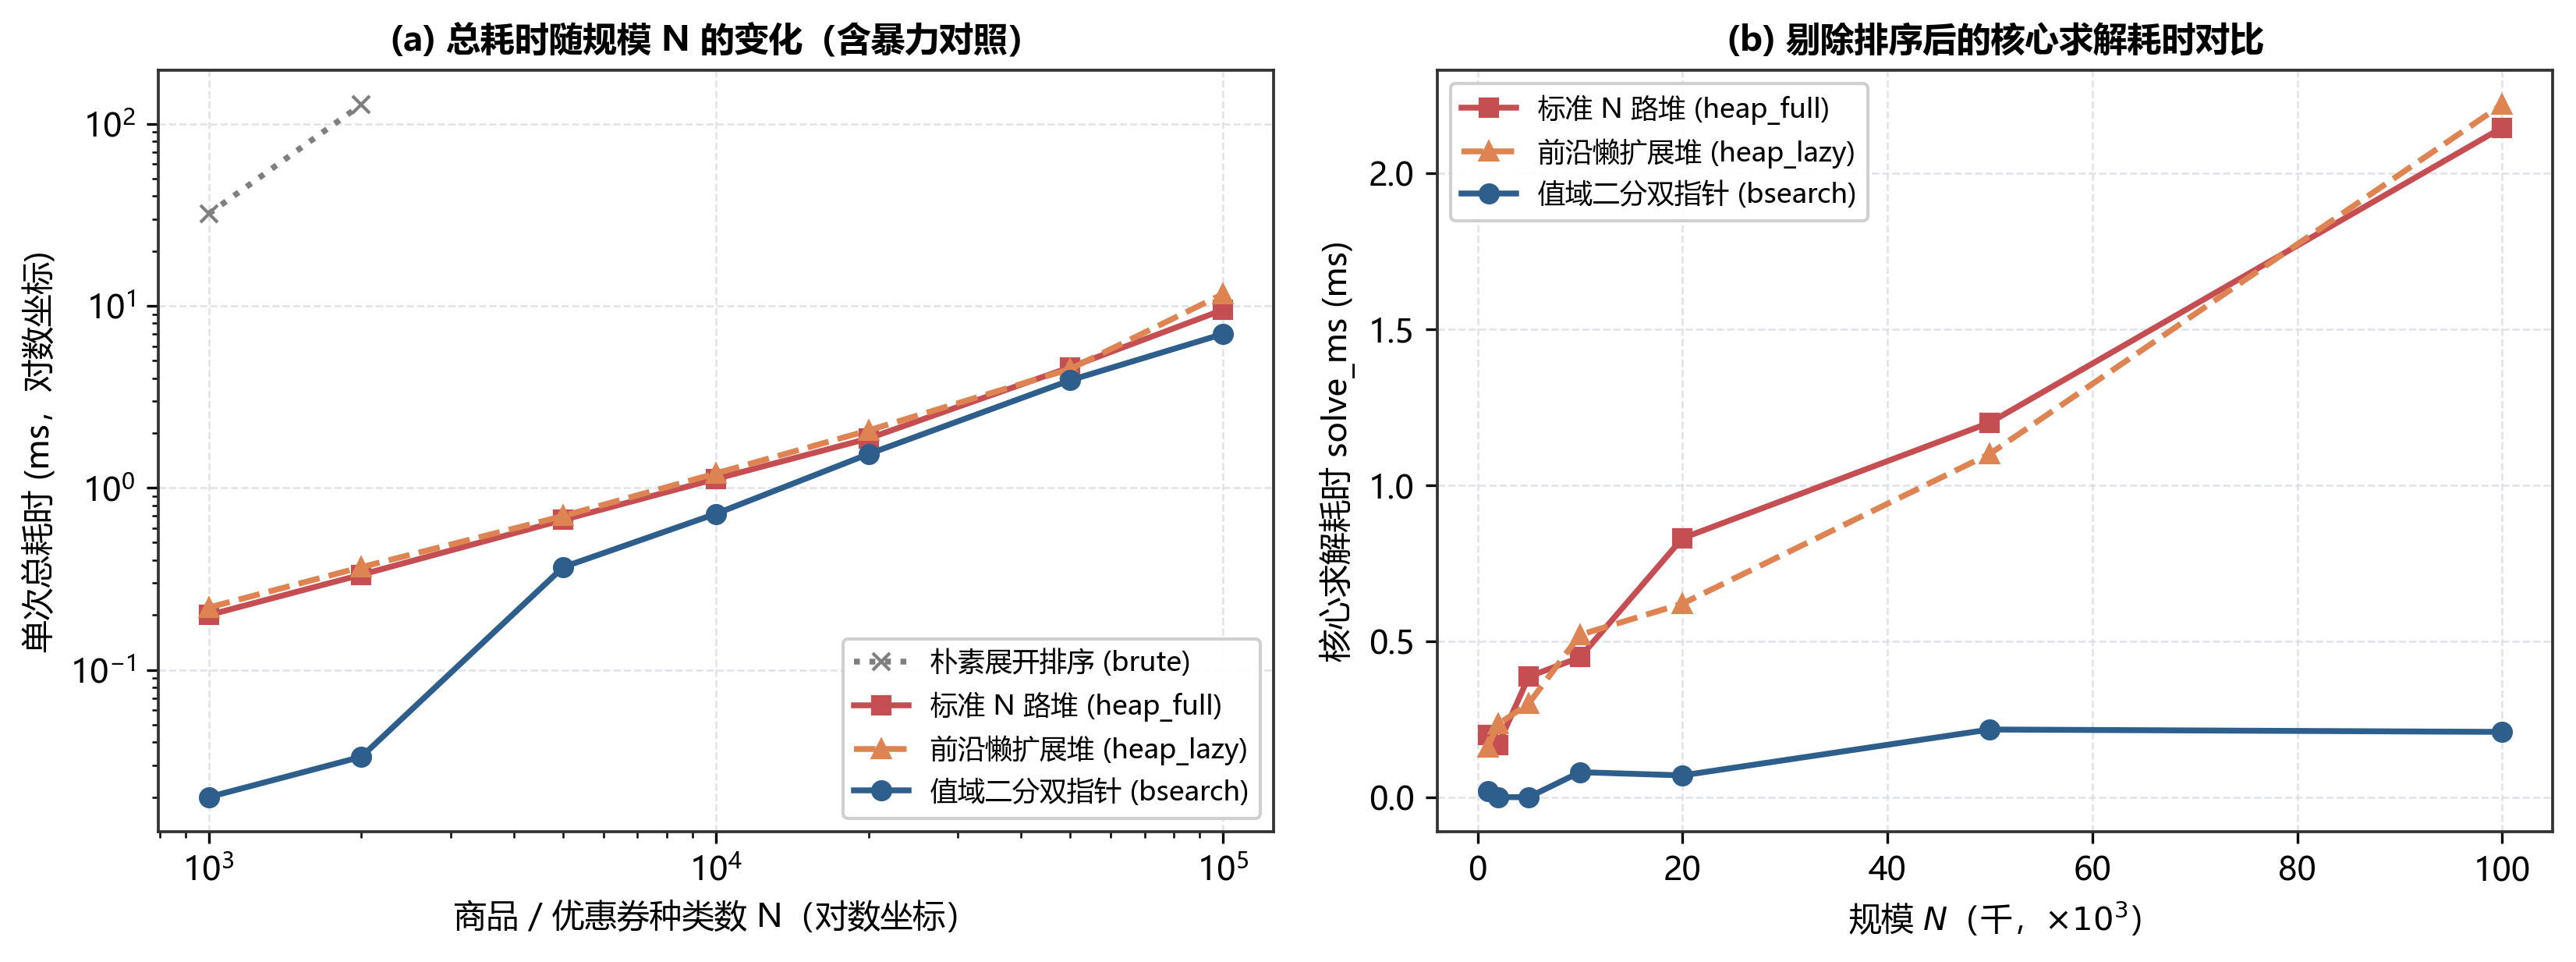
\includegraphics[width=0.98\textwidth]{results/figures/fig1_scale.png}
\caption{实验族 A：规模 $N$ 从 $10^3$ 增至 $10^5$ 时的总耗时 (a) 与剔除排序后的核心求解耗时 (b)}
\label{fig:scale}
\end{figure}

表~\ref{tab:scale} 中，\code{brute} 在 $N=2000$ 时已达 127.33~ms，比 \code{bsearch} 慢超过三千倍，耗时几乎全在 $4\times 10^6$ 个配对的排序上。在 $N=10^5, K=629\,285$ 时，三个高效算法总耗时落在 7.0--11.6~ms；剔除排序后差距立刻拉开：\code{bsearch} 仅需 0.21~ms，比 \code{heap\_full}（2.15~ms）与 \code{heap\_lazy}（2.22~ms）快超过 10 倍。

实验族 B 固定 $N=10^5, D=10^6$，通过改变实付价区间将实际购买件数 $K$ 从 111 扫到 $10^6$，实测见表~\ref{tab:ksweep} 与图~\ref{fig:ksweep}。

\begin{table}[htbp]
\centering
\caption{实验族 B：购买量 $K$ 梯度实测（$N=10^5, D=10^6$，列值为核心求解耗时 \code{solve\_ms} / 步数 \code{ops}）}
\label{tab:ksweep}
\footnotesize
\begin{tabular}{@{}lrccc@{}}
\toprule
\rowcolor{gray!12}\tabhead{档位} & \tabhead{件数 $K$} & \tabhead{\code{heap\_full}} & \tabhead{\code{heap\_lazy}} & \tabhead{\code{bsearch}} \\
\midrule
\code{K1\_tiny}   & 111        & 0.51 ms / 100K  & 0.00 ms / 118   & 0.10 ms / 1.20M \\
\code{K2\_small}  & 1\,248     & 0.31 ms / 101K  & 0.00 ms / 1.5K  & 0.31 ms / 1.30M \\
\code{K3\_mid1}   & 19\,470    & 0.41 ms / 121K  & 0.00 ms / 21K   & 0.10 ms / 1.20M \\
\code{K4\_mid2}   & 94\,517    & 0.52 ms / 197K  & 0.30 ms / 97K   & 0.51 ms / 1.00M \\
\code{K5\_large}  & 630\,295   & 1.72 ms / 740K  & 1.58 ms / 640K  & 0.10 ms / 0.90M \\
\code{K6\_xlarge} & 1\,000\,000 & 2.53 ms / 1.10M & 2.13 ms / 1.00M & 0.00 ms / 0.51M \\
\code{K7\_max1e6} & 1\,000\,000 & 2.43 ms / 1.10M & 2.54 ms / 1.00M & 0.11 ms / 0.20M \\
\bottomrule
\end{tabular}
\end{table}

\begin{figure}[htbp]
\centering
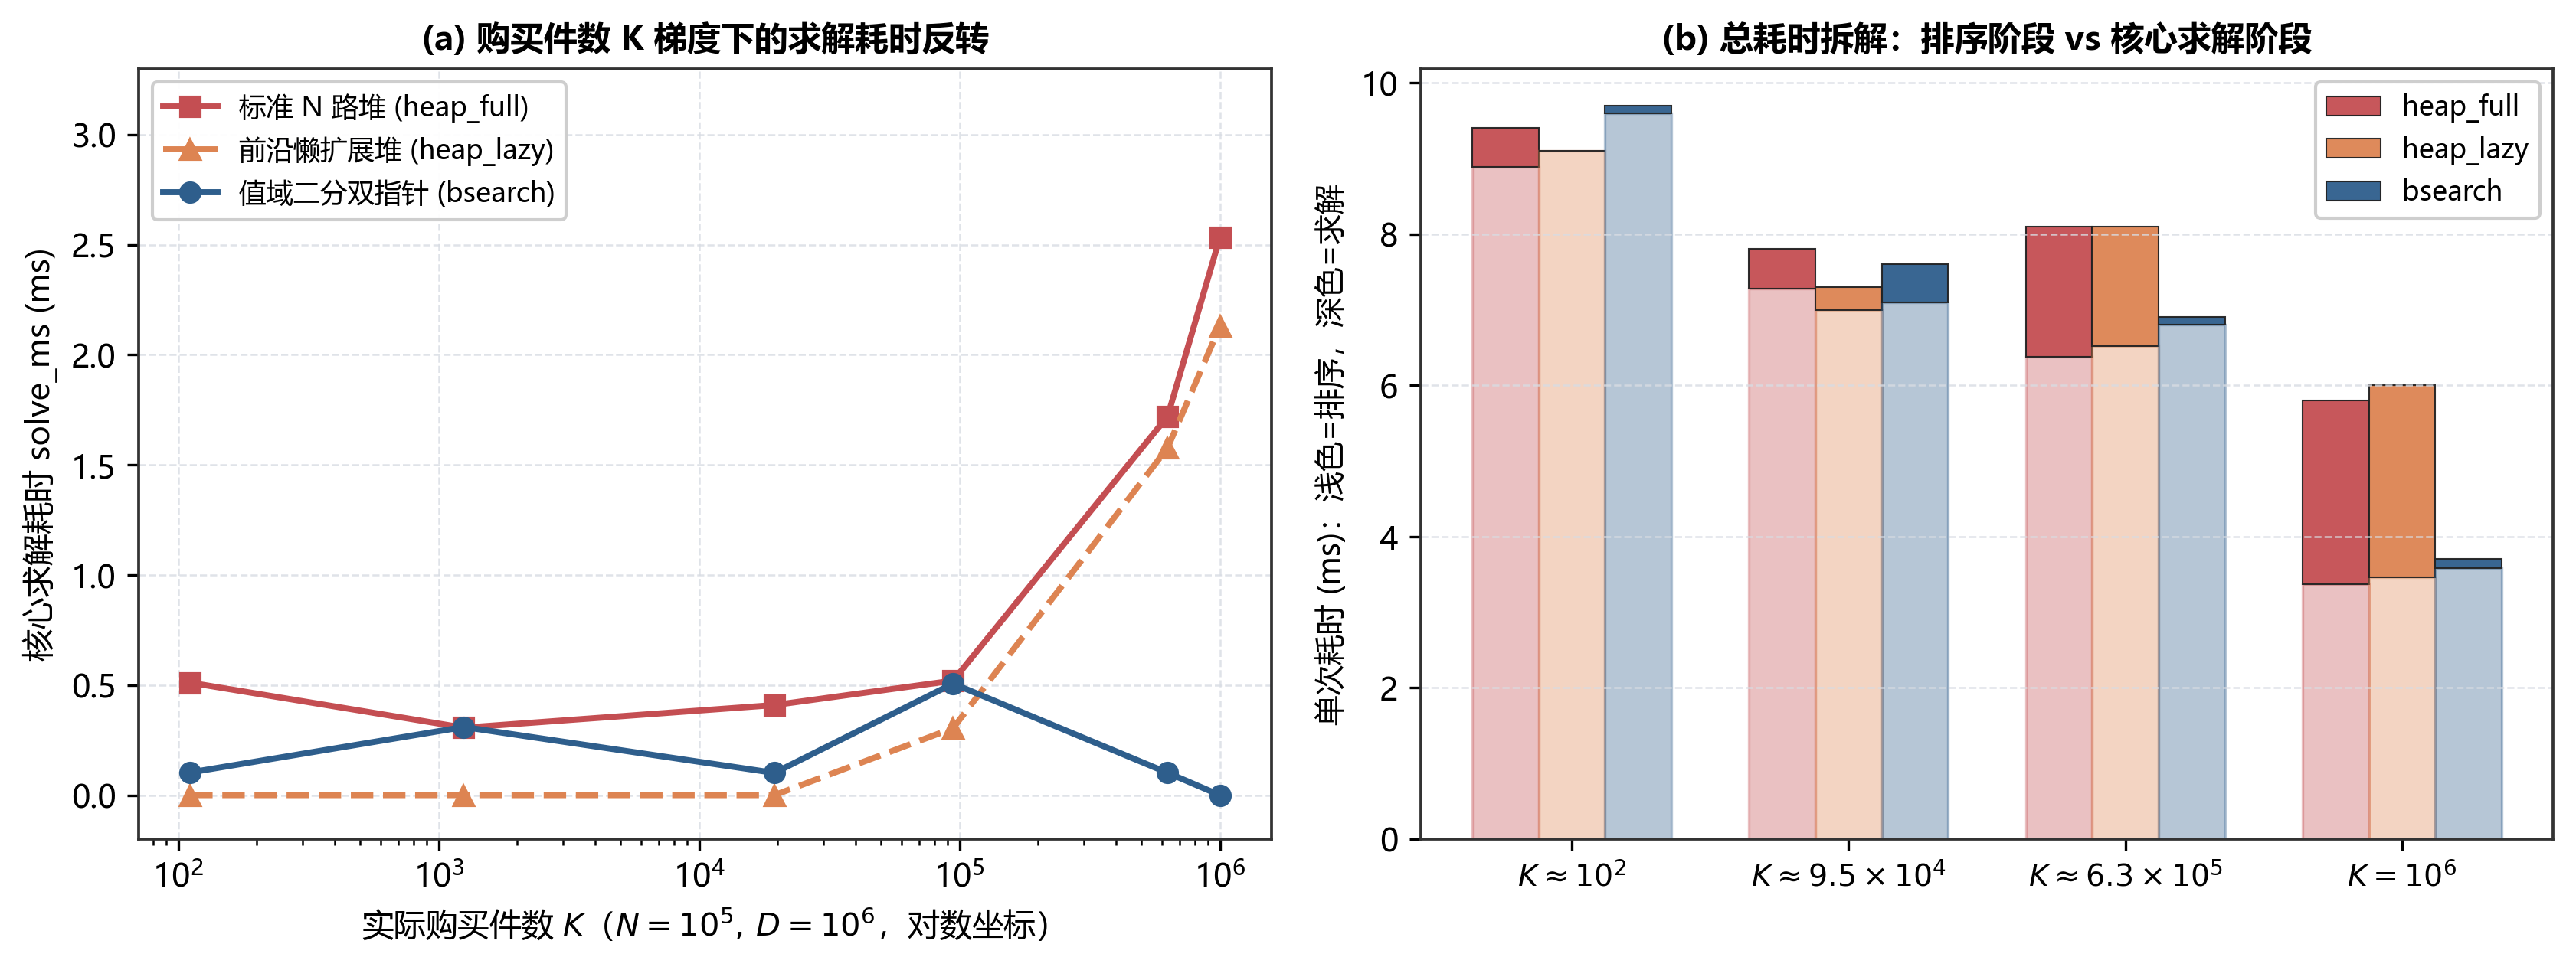
\includegraphics[width=0.98\textwidth]{results/figures/fig2_k_sweep.png}
\caption{实验族 B：核心求解耗时随购买件数 $K$ 的反转 (a) 与排序/求解占比拆解 (b)}
\label{fig:ksweep}
\end{figure}

当 $K \le 9.5\times 10^4$（\code{K1}--\code{K4}）时，\code{heap\_lazy} 核心步数在百级到十万级，求解耗时仅 0.00--0.30~ms，快过 \code{heap\_full} 与 \code{bsearch}。跨过 $10^5$ 后（\code{K5}--\code{K7}），两类堆的求解耗时升至 1.58--2.54~ms，而 \code{bsearch} 压在 0.00--0.11~ms，领先超过一个数量级。图~\ref{fig:ksweep}(b) 同时给出总耗时拆解：在 \code{K1}--\code{K4} 上，两次排序占三个算法总耗时的 93\%--100\%；到 \code{K5} 仍占 79\%--99\%。

\subsection{分布敏感度与超大预算拓展实验}

实验族 C 在 $N=10^5, D=10^6$ 下测五种分布，结果见表~\ref{tab:dist}。在高价低购买量的 \code{D2\_uniform\_exp}（$K=492$）上，\code{heap\_lazy} 求解耗时落到 0.00~ms（776 步）；在全相等平地 \code{D3\_all\_equal} 与阶梯离散 \code{D4\_step\_3levels} 上，\code{bsearch} 分别仅需 0.08~ms（0 轮二分直接收尾）与 0.22~ms，而两类堆在 \code{D4} 上要弹满 100 万次，用掉 2.53--2.77~ms。

\begin{table}[htbp]
\centering
\caption{实验族 C：五种典型分布下的核心求解耗时与轮数（$N=10^5, D=10^6$）}
\label{tab:dist}
\footnotesize
\begin{tabular}{@{}lrccc@{}}
\toprule
\rowcolor{gray!12}\tabhead{分布用例} & \tabhead{件数 $K$} & \tabhead{\code{heap\_full} (ms)} & \tabhead{\code{heap\_lazy} (ms)} & \tabhead{\code{bsearch} (ms / 轮)} \\
\midrule
\code{D1\_uniform\_cheap} & 278\,552   & 0.93 & 0.52 & 0.72 / 11 \\
\code{D2\_uniform\_exp}   & 492        & 0.41 & 0.00 & 0.81 / 19 \\
\code{D3\_all\_equal}     & 200\,000   & 0.90 & 0.44 & 0.08 / 0 \\
\code{D4\_step\_3levels}  & 1\,000\,000 & 2.77 & 2.53 & 0.22 / 19 \\
\code{D5\_heavy\_gap}     & 178\,629   & 0.91 & 0.41 & 0.31 / 20 \\
\bottomrule
\end{tabular}
\end{table}

实验族 D 突破题面 $D \le 10^6$ 上限，固定 $N=10^5$ 将预算推高至 $10^{14}$（表~\ref{tab:huge_budget}、图~\ref{fig:huge_budget}）。在 $D=10^6$ 时 \code{heap\_lazy} 略占优（0.21~ms 对 0.52~ms）；到 $D=10^7$（$K=48\,909$）时 \code{bsearch} 开始反超；到 $D=10^{10}$（$K=4\,811\,922$）时，两类堆的核心耗时飙升到 132.0--140.5~ms，比 \code{bsearch}（1.56~ms）慢了 85--90 倍；到 $D=10^{14}$（$K \approx 22.33$ 亿）时，按堆每百万次弹出约 28~ms 外推至少需要一分钟以上，而 \code{bsearch} 仅需 20.7~ms（求解段 9.85~ms）。

\begin{table}[htbp]
\centering
\caption{实验族 D：超大预算拓展（$N=10^5$，$D$ 推高至 $10^{14}$；总耗时 / 求解耗时，单位 ms）}
\label{tab:huge_budget}
\footnotesize
\begin{tabular}{@{}rrccc@{}}
\toprule
\rowcolor{gray!12}\tabhead{预算 $D$} & \tabhead{实际购买件数 $K$} & \tabhead{\code{heap\_full}} & \tabhead{\code{heap\_lazy}} & \tabhead{\code{bsearch}} \\
\midrule
$10^6$    & 10\,479         & 10.9 / 0.30    & 10.8 / 0.21    & 11.3 / 0.52 \\
$10^7$    & 48\,909         & 12.0 / 1.20    & 11.7 / 0.92    & 11.6 / 0.61 \\
$10^8$    & 224\,327        & 16.6 / 5.60    & 16.0 / 5.06    & 11.4 / 0.21 \\
$10^{10}$ & 4\,811\,922     & 151.0 / 140.50 & 143.0 / 131.96 & 13.5 / 1.56 \\
$10^{12}$ & 103\,492\,063   & ---            & ---            & 13.3 / 2.06 \\
$10^{14}$ & 2\,233\,468\,109 & ---            & ---            & 20.7 / 9.85 \\
\bottomrule
\end{tabular}
\end{table}

\begin{figure}[htbp]
\centering
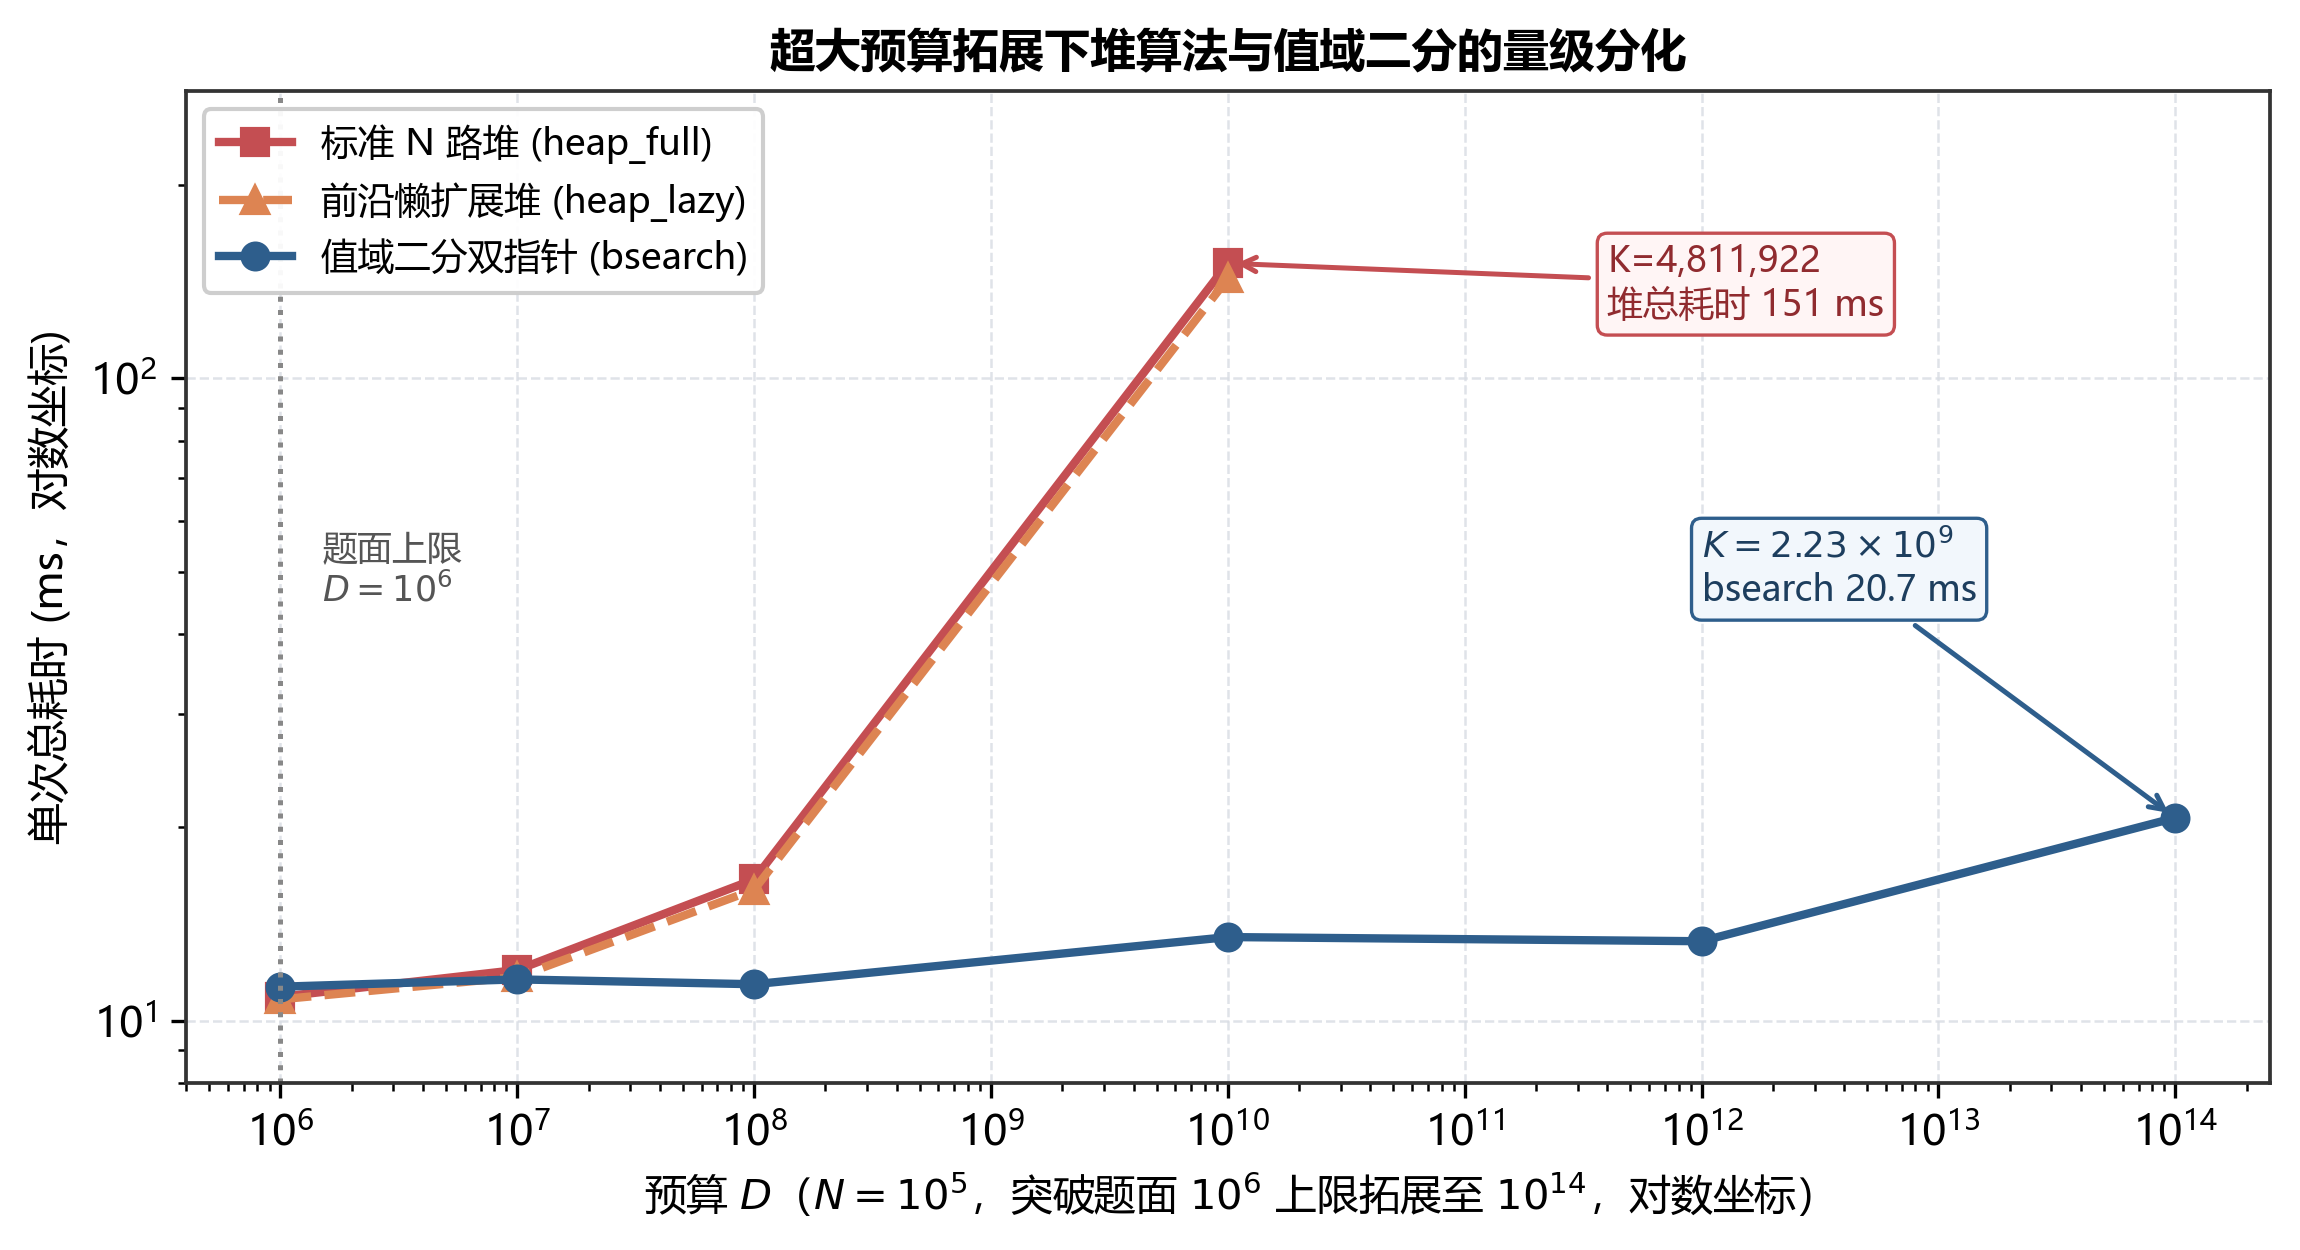
\includegraphics[width=0.78\textwidth]{results/figures/fig3_huge_budget.png}
\caption{实验族 D：突破题面 $D \le 10^6$ 限制后，堆算法与值域二分的量级分化}
\label{fig:huge_budget}
\end{figure}

%=====================================================================
\section{Analysis and Comments}

\subsection{时间与空间复杂度推导}

本节逐一推导四个求解器的渐近阶与内存占用（容量按二进制 $1~\text{MiB}=2^{20}$~B、$1~\text{GiB}=2^{30}$~B 换算）。

\begin{enumerate}[leftmargin=1.6em,itemsep=0.3em,topsep=0.18em]
  \item \textbf{\code{brute}：}生成 $N^2$ 个实付价需 $\Theta(N^2)$，全排序需 $\Theta(N^2\log(N^2)) = \Theta(N^2\log N)$，扫描至多 $N^2$ 步；总时间 $\Theta(N^2\log N)$。数组 \code{all} 存 $N^2$ 个 8 字节整数，空间 $\Theta(N^2)$，$N=10^5$ 时约 74.5~GiB。

  \item \textbf{\code{heap\_full}：}两次排序需 $O(N\log N)$，有序行首线性装堆耗时 $\Theta(N)$；主循环共弹出 $K \le \min(N^2, D)$ 次，每次下沉深度至多 $\lfloor \log_2 N \rfloor$，总时间 $O(N\log N + K\log N)$。空间为拷贝数组 $p, c$（共 $16N$~B）加 1-indexed 堆数组（每结点 16~B，共 $16N$~B），合计约 $32N$~B（$N=10^5$ 时约 3.05~MiB），阶为 $O(N)$。

  \item \textbf{\code{heap\_lazy}：}排序同为 $O(N\log N)$。每轮弹出 $(r, col)$ 至多让堆净增 1 个结点，且每行至多有一个活跃前沿在堆里，故堆上限 $H_{\max} \le \min(N, K+1)$。核心求解时间 $O(K\log\min(N, K))$，总时间 $O(N\log N + K\log\min(N, K))$。堆本身占 $O(\min(N, K))$，连同输入排序数组总空间 $O(N)$。

  \item \textbf{\code{bsearch}：}排序 $O(N\log N)$，构建 \code{prefC} 需 $\Theta(N)$。在 \code{checkBudget(T)} 中，外层 $i$ 最多迭代 $N$ 次，内层指针 $j$ 从 $N-1$ 只减不增、总左移次数至多 $N$ 次，单次判定严格 $O(N)$。二分搜索区间含至多 $\min(V, D)$ 个整数，轮数不超过 $\lceil \log_2(\min(V, D)+1) \rceil$，加末尾一次完整扫描，总时间 $O(N\log N + N\log(\min(V, D)+1))$。空间为 $p, c$（$16N$~B）加 16 字节宽 \code{prefC}（$16N$~B），合计约 $32N$~B（$N=10^5$ 时约 3.05~MiB），阶为 $O(N)$。
\end{enumerate}

\subsection{实测性能拆解：排序瓶颈、反转机制与单步代价}

\textbf{第一，题面常规约束下的主要耗时落在排序上。}在实验族 B（图~\ref{fig:ksweep}(b)）的 \code{K1}--\code{K4} 档位上，$N=10^5$ 的两次 \code{std::sort} 耗时 7.0--9.6~ms，占总耗时的 93\%--100\%；而 \code{bsearch} 核心求解全程不到 0.55~ms。同时，\code{K7\_max1e6} 与 \code{D3\_all\_equal} 的 $N$ 同样是 $10^5$，排序却缩至 3.4--3.6~ms 与 1.1--1.5~ms，原因是两者仅有极少数不同取值，GCC 的 Introsort 在大量重复键上更快收敛。不拆分 \code{sort\_ms} 与 \code{solve\_ms}，直接拿不同输入的总耗时比大小就会被排序敏感性误导。

\textbf{第二，$K$ 梯度反转是「随机堆访存」与「顺序扫描」的交叉。}在 $K \le 9.5\times 10^4$ 时，\code{heap\_lazy} 总步数仅 118 到 9.7 万，比 \code{bsearch} 少一到四个数量级，求解耗时压在 0.30~ms 内；\code{heap\_full} 需先装满 $10^5$ 个行首，白多出 10 万次写入。跨过 $K \approx 10^5$ 后，堆每次下沉在数组里按 \code{idx<<1} 跨缓存行跳跃，步数随 $K$ 飙升至百万以上，而 \code{bsearch} 顺序扫描连续数组 $p, c$ 吃满硬件预取，在 $K=10^6$ 时拉开超过十倍、在 $D=10^{10}$ 时拉开 85--90 倍差距。

\textbf{第三，同一算法内不同指令的单步代价差。}在实验族 D 的 \code{bsearch} 上，从 \code{B1}（$D=10^6$）到 \code{B6}（$D=10^{14}$），\code{ops} 只从 180 万涨到 302 万（1.67 倍），求解耗时却从 0.52~ms 涨到 9.85~ms（19 倍）。对照 \code{checkBudget} 代码即可看清：在 \code{B1}--\code{B4} 上，180 万步里绝大多数是每轮第 0 行把 $j$ 从 $99\,999$ 线性退回几百的纯减法空转，后面几十行随即触发 \code{p[i]-c[0]>T} 退出；到了 $D=10^{14}$（买下全矩阵 22\% 的格子），每轮都要跑满全部 10 万行，每行执行一次 128 位乘加与跨度较大的 \code{prefC[m]} 访存（1.53~MiB 跨出 L2 缓存）。同一计数器把内层纯减法与外层 128 位乘加和访存混为一谈，导致倍率对不齐。这同时给出一条直接的工程改进：进入行循环前对第 0 行做一次 \code{upper\_bound}（$O(\log N)$）定位初始 $j$，即可砍掉低预算下的线性回退。

\subsection{模型变体拓展}

在实际场景中，围绕优惠券使用规则常有两类容易混淆的变体，这里简要对比它们如何改变算法结构：

\begin{itemize}[leftmargin=1.6em,itemsep=0.18em,topsep=0.18em]
  \item \textbf{变体一：允许不使用优惠券按原价购买。}若每种商品至多无券买一次，等价于往优惠券集合加入一张面值为 0 的虚拟券，矩阵变为 $N\times(N+1)$，本文全部算法与证明原样成立；若允许同一商品无券无限购买，由于 $p_i - c_j < p_i$，无券原价只会在 $N^2$ 个带券配对买光之后才被启用，只需在全买光分支后用余钱整除 $\min p_i$ 即可。
  \item \textbf{变体二：每种优惠券全局限用一次、每种商品限买一次。}此时配对空间从二维矩阵坍缩为一维匹配：买 $k$ 件的最优方案必取最便宜的 $k$ 件商品配面值最大的 $k$ 张券，排序后单趟扫前缀和即可 $O(N\log N)$ 解决，与本题的二维归并或值域二分结构完全不同。
\end{itemize}

\subsection{结论}

\begin{enumerate}[leftmargin=1.8em,itemsep=0.18em,topsep=0.18em]
  \item 实付价格矩阵的行列单调性与 $M[i][j] \ge 1$ 给出上界 $K \le \min(N^2, D)$，使优先队列在题面约束内可行，也划出了它在大预算下的失效边界。
  \item 在满规模 $N=10^5, D=10^6$ 下，购买量 $K$ 决定求解阶段排名：\code{heap\_lazy} 在 $K \le 9.5\times 10^4$ 最快（$\le 0.30$~ms），\code{bsearch} 跨过 $K \approx 10^5$ 后稳固领先并在 $K=10^6$ 压到 0.00--0.11~ms；同时排序在 \code{K1}--\code{K4} 上占总耗时的 93\%--100\%。
  \item 预算扩至 $D \gg 10^6$ 后，两类堆随 $K$ 按 $O(K\log N)$ 级迅速膨胀（$D=10^{10}$ 时求解需 132--141~ms，$D=10^{14}$ 不可行），而 \code{bsearch} 在买下 22.33 亿件时总耗时仅 20.7~ms，故默认评测模式选用 \code{bsearch}。
  \item \textbf{适用边界：}上述实测耗时与 $K \approx 10^5$ 交叉点仅对本机 GCC \code{-O2}、64 位整数输入及本文四族测试分布成立；同时值域二分依赖价格为离散整数，若题目改作任意精度实数价格，则无法在实数域上做整数值域二分。
\end{enumerate}

\subsection{局限}

\begin{enumerate}[leftmargin=1.8em,itemsep=0.18em,topsep=0.18em]
  \item 计时基于 1~ms 粒度的 \code{clock()}；虽经多轮重复平滑，对单次低于 0.05~ms 的极小规模测试（如 $N \le 5000$ 或小 $K$ 下的 \code{heap\_lazy} 与 \code{bsearch} 求解段）仍无法分辨微秒级差异。
  \item 缺乏官方隐藏测试集，360 组对拍与四大实验族均由固定种子脚本生成，未必覆盖线上评测的全部对抗分布。
  \item 内存占用按容器元素字节数与规模上限理论推算，未接入系统级峰值内存采样工具实测。
  \item 操作计数器 \code{ops} 仅记录最内层循环步数、未按指令权重归一化（如 4.2 节所述，在 \code{bsearch} 中混入了第 0 行纯减法与外层 128 位乘加），不能直接跨算法换算耗时倍率。
  \item 4.2 节提出的「第 0 行改用 \code{upper\_bound} 定位初始 $j$」优化目前仅是事后机制推论，尚未合入代码做前后对照测量。
\end{enumerate}

%=====================================================================
\renewcommand{\refname}{References}
\begin{thebibliography}{9}
\small
\setlength{\itemsep}{2pt}
\bibitem{clrs2022} T. H. Cormen, C. E. Leiserson, R. L. Rivest, C. Stein, ``Introduction to Algorithms'', MIT Press, 4th edition, (2022)
\bibitem{knuth1998} D. E. Knuth, ``The Art of Computer Programming, Volume 3: Sorting and Searching'', Addison-Wesley, 2nd edition, (1998)
\end{thebibliography}

%=====================================================================
\clearpage
\section*{Author List}

\vspace{0.2em}
\begin{center}
\begin{tabular}{@{}>{\raggedright\arraybackslash}p{2.6cm}>{\raggedright\arraybackslash}p{11.4cm}@{}}
\toprule
\rowcolor{gray!12}\tabhead{成员} & \tabhead{负责的内容} \\
\midrule
Member A & 数学建模与贪心/收尾定理证明，四种求解器（暴力、两类最小堆、值域二分双指针）的统一接口与核心实现，报告第 1--2 章与第 4 章撰写 \\
Member B & 四层自动对拍与边界用例构造，四大基准实验族脚本编写、批量测速与图表绘制，报告第 3 章整理、版式校对与匿名提交包自检 \\
\bottomrule
\end{tabular}
\end{center}

\vspace{1.8em}

\section*{Declaration}

\noindent
We hereby declare that all the work done in this project titled ``Shopping With Coupons: Heap Merging and Value-Domain Binary Search'' is of our independent effort as a group.

\vspace{2.2em}
\section*{Signatures}

\vspace{1.8em}
\begin{center}
\begin{tabular}{@{}c@{\hspace{2.4cm}}c@{}}
\rule{5.2cm}{0.4pt} & \rule{5.2cm}{0.4pt} \\[0.4em]
Member A & Member B \\[0.3em]
Date: \rule{2.8cm}{0.4pt} & Date: \rule{2.8cm}{0.4pt} \\
\end{tabular}
\end{center}

\end{document}
